\ifdefined\XeTeXversion\else\pdfoutput=1\fi
\documentclass[12pt]{article}

\usepackage[margin=1in]{geometry}
\usepackage{amsmath}
\usepackage{mathptmx}
\usepackage{setspace}
\usepackage{graphicx}
\usepackage{booktabs}
\usepackage[hidelinks]{hyperref}
\usepackage{url}
\urlstyle{same}

\doublespacing

\title{Memory Is the Price: Evidence from the LLM Serving Market on the
Economics of Mixture-of-Experts Inference\\[4pt]
\large (Extended Abstract)}

\author{Michael J.\ Yuan (ByteFuture Inc.) \and Ju Long (Texas State University)}

\date{}

\begin{document}
\maketitle

\vspace{0.5em}
\noindent\textbf{Abstract.} Sparse Mixture-of-Experts (MoE) models are widely
claimed to cost what their \emph{active} compute costs. We test this claim
against the LLM serving market itself. Because providers disclose almost
nothing about their production systems, we treat posted prices as an
observable proxy for the latent serving configuration. A hedonic regression
over 289 provider--model price observations (38 models, 2026-07-06) rejects
the claim: the market bills MoE models most of the way toward their total
memory footprint (sparsity elasticity 0.481, $t = 4.9$,
$p = 1.9 \times 10^{-5}$). Market structure supports the scale reading: the price floor of every
200B+ panel belongs to a vertically integrated provider, never to a
general-purpose cloud, hyperscalers price 1.2--8.8$\times$ above the floor,
and MoE price dispersion remains compressed, consistent with selective
listing. DeepSeek, whose vendor anchors its own
serving prices, is excluded from the primary panel and analyzed separately:
its sparse-attention generation is served at roughly one fifth of the
market schedule.

\section{Motivation: an efficiency claim the market can test}

Frontier open-weight language models have shifted decisively to sparse MoE
architectures, which store hundreds of billions of parameters but activate
only a small fraction per token: DeepSeek-R1 activates 37B of 671B, and Kimi
K2 activates 32B of one trillion. The architecture's economic pitch is that
customers pay only for active compute. Switch Transformers promised ``outrageous numbers of parameters'' at ``a constant computational cost''~\cite{fedus}, and Mistral stated that Mixtral ``processes input and
generates output at the same speed and for the same cost'' as a dense model
the size of its active parameters~\cite{mistral}.

Whether the market delivers this discount is difficult to check directly,
because commercial inference is an unusually opaque industry. Providers
publish per-token prices, but almost never the cluster scale, parallelism,
served precision, batch size, utilization, or margin of any endpoint, and
black-box audits show that 11 of 31 commercial Llama endpoints served output
distributions deviating from the reference weights~\cite{gao}. The serving
configuration is thus a latent variable, and the posted price is its
observable proxy. Open-weight serving approximates the textbook competitive case: the weights are free, the software is open source, entry is unrestricted, and dozens of providers quote side by side on the OpenRouter marketplace. Competition therefore disciplines prices toward marginal cost, and sustained price structure identifies cost structure~\cite{hayek}.

\section{Hypotheses}

Our empirical strategy follows the hedonic-pricing tradition~\cite{rosen}: we
regress prices on the characteristics that drive resource consumption and
read the coefficients as the market's implicit prices for each resource. In
\begin{equation}
\log(\text{price}) = c_0 + c_1 \log(\text{active\_params})
                        + c_2 \log(\text{total}/\text{active}),
\label{eq:hedonic}
\end{equation}
$c_1$ values active compute and $c_2$ values resident-but-inactive capacity.
\textbf{H1 (compute pricing, the industry claim)} predicts $c_2 = 0$; if
memory rather than compute is the binding cost, $c_2 \approx c_1$.
\textbf{H2 (scale economies)} holds that the minimum efficient scale of large
MoE serving exceeds a single node, because the compute savings are only
captured when traffic from thousands of users is aggregated across
expert-parallel decoding pools~\cite{deepseek,lmsys}. H2 predicts that price
floors are set by massively parallel ``neocloud'' providers, that
general-purpose clouds price above them, and that providers who cannot
justify such pools exit rather than list, which compresses observed price
dispersion through selection~\cite{heckman}.

\section{Data and method}

We collected the complete endpoint listings for 129 candidate open-weight
models from OpenRouter's public endpoints API on 2026-07-06, cross-checked
against provider price pages. After mechanical exclusions and a
three-provider threshold, 46 models qualify. The seven DeepSeek panels are
excluded on identifying-assumption grounds, because the vendor anchors its
own prices. The primary panel comprises 289 observations across 38 models
(28 MoE, 10 dense) from 42 providers, joined to architecture parameters
verified against each model's HuggingFace repository. All statistics are computed deterministically; the data
and code are public.\footnote{\url{https://github.com/juntao/memory_is_the_price}}

\section{Results}

\textbf{H1 is rejected.} The sparsity ratio, which compute pricing predicts
to be free, is priced at 84\% of the rate of active compute
(Table~\ref{tab:ols}). A 1{,}000B-total/32B-active model is billed like a
$\sim$580B dense model, and the median MoE model sits 5$\times$ above the
dense-only price schedule (Figure~\ref{fig:level}). Customers keep little
of the advertised discount.

\begin{table}[h]
\centering
\begin{singlespace}
\caption{The table reports OLS estimates of regression~\eqref{eq:hedonic}
($n = 38$ models, $R^2 = 0.490$, $F(2,35) = 16.8$,
$p = 7.7 \times 10^{-6}$). H1 predicts $c_2 = 0$; the measured ratio is
$c_2/c_1 = 0.84$.}
\label{tab:ols}
\begin{tabular}{lrrrr}
\toprule
Coefficient & Estimate & Std.\ err. & $t$ & $p$ \\
\midrule
$c_1$: log(active parameters) & $+0.572$ & 0.138 & 4.1 & $2.1 \times 10^{-4}$ \\
$c_2$: log(total/active)      & $+0.481$ & 0.097 & 4.9 & $1.9 \times 10^{-5}$ \\
\bottomrule
\end{tabular}
\end{singlespace}
\end{table}

\begin{figure}[h]
\centering
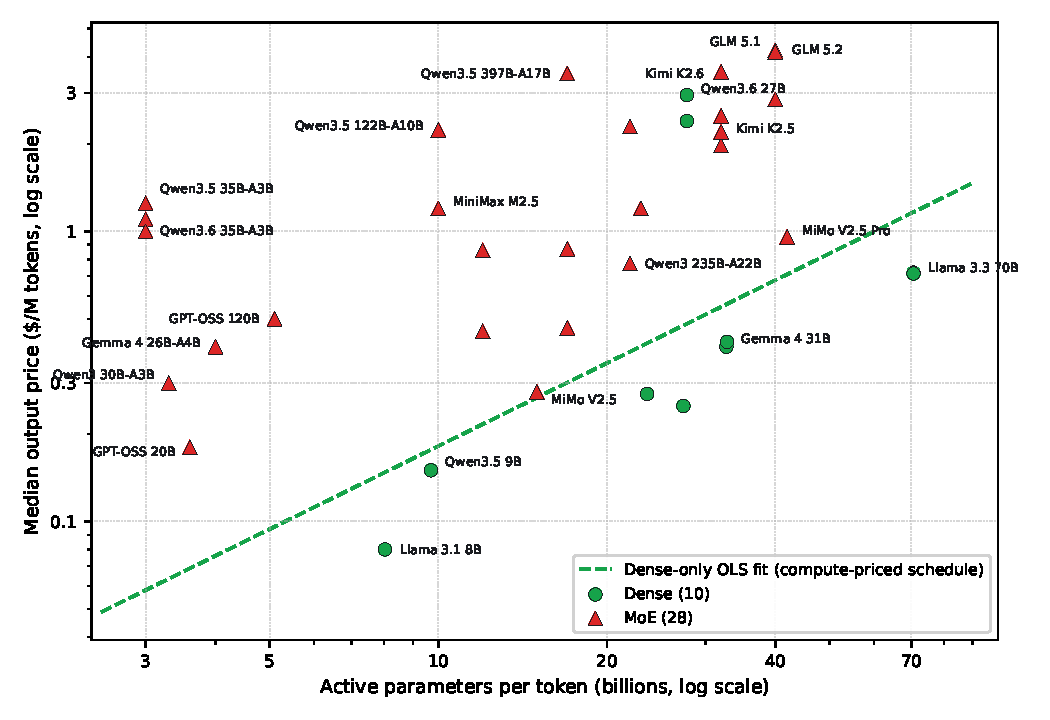
\includegraphics[width=0.82\linewidth]{fig1_price_level.pdf}
\begin{singlespace}
\caption{The figure plots median output price against active parameters for
the 38 primary-panel models on log-log axes. The median MoE model (triangle) sits 5$\times$ above the
dense-only OLS fit (dashed line), which is the schedule a compute-priced
market would apply.}
\label{fig:level}
\end{singlespace}
\end{figure}

\textbf{H2 is supported.} Published deployments show a
$\sim$36$\times$ per-GPU decode throughput gap between a 96-GPU
expert-parallel pool and a single 8-GPU node, so no provider can sell at the
pool's marginal cost from a single-node
deployment~\cite{lmsys,dzhsurf}. In all seventeen panels for models of 200B+
total parameters, the floor is set by a vertically integrated provider, a
neocloud in eleven and the model's owner in six; no general-purpose cloud
sets a floor, and hyperscaler listings sit 1.2--8.8$\times$ above it.
Participation counts are not used as a test, because they are confounded by
demand for newer models. MoE price dispersion remains \emph{compressed}
rather than widened (median coefficient of variation 0.23 versus 0.35 for
dense): providers whose latent cost exceeds the competitive price tend not
to list, so the observed prices are a selected sample~\cite{heckman}. The
excluded DeepSeek panels sharpen the mechanism: the vendor's
sparse-attention generation is served at roughly one fifth of the schedule
by a dozen third parties, and DeepSeek itself floors its flagship
3.6$\times$ below the third-party median.

\section{Contribution and implications}

To our knowledge this paper provides the first hedonic estimate of the sparsity elasticity of price, formalizing an observation made informally on five models by Scher~\cite{scher} and raised descriptively by Li et al.~\cite{li}. It also provides the first market-structure evidence that large-MoE serving is gated by scale. For information-systems and economics audiences, the study
demonstrates a general method: using marketplace prices as revealed cost
structure for digital infrastructure whose production technology is
deliberately undisclosed. For practitioners, the results imply that MoE
serving economics are governed by memory rather than FLOPS, and that the
economically rational serving hardware outside hyperscale pools inverts the
GPU design point: large commodity memory, modest compute, and moderate
bandwidth.

\begin{thebibliography}{9}
\bibitem{fedus} Fedus, W., Zoph, B., \& Shazeer, N. Switch Transformers:
scaling to trillion parameter models with simple and efficient sparsity.
arXiv:2101.03961, 2021.
\bibitem{mistral} Mistral AI. Mixtral of experts. 2023-12-11.
\url{https://mistral.ai/news/mixtral-of-experts/}
\bibitem{gao} Gao, I., Liang, P., \& Guestrin, C. Model equality testing:
which model is this API serving? ICLR 2025. arXiv:2410.20247.
\bibitem{hayek} Hayek, F.~A. The use of knowledge in society. \emph{American
Economic Review} 35(4), 519--530, 1945.
\bibitem{rosen} Rosen, S. Hedonic prices and implicit markets: product
differentiation in pure competition. \emph{Journal of Political Economy}
82(1), 34--55, 1974.
\bibitem{deepseek} DeepSeek-AI. DeepSeek-V3/R1 inference system overview.
Open Infra Index, 2025.
\bibitem{lmsys} LMSYS. Deploying DeepSeek with PD disaggregation and
large-scale expert parallelism on 96 H100 GPUs. 2025-05-05.
\bibitem{heckman} Heckman, J.~J. Sample selection bias as a specification
error. \emph{Econometrica} 47(1), 153--161, 1979.
\bibitem{dzhsurf} dzhsurf. DeepSeek V3/R1 deployment benchmarks, 8$\times$H100
(AWQ 4-bit, vLLM). \url{https://github.com/dzhsurf/deepseek-v3-r1-deploy-and-benchmarks}
\bibitem{scher} Scher, A. Observations about LLM inference pricing. MIRI
Technical Governance Team blog, 2025-03-03.
\bibitem{li} Li, H., et al. When is the same model not the same service?
arXiv:2605.02821, 2026.
\end{thebibliography}

\end{document}
